\chapter{Message Passing Interface}
%In this chapter, we will introduce our \gls{mpi} library.

To be able to simulate radio communication using \gls{mpi}, it is necessary to expose a series of functions, such that \gls{manet} nodes will be able to communicate with each other. This will be done in three parts. The first part is a set of hardware emulating functions to enable transmission and reception of data packets between nodes. This part is introduced in \autoref{sec:mpiprotocol}. The second part is a centralised controller, used to control the networking between the nodes. The controller is presented in \autoref{sec:mpicontroller}. The third part is the \acrfull{lmc}, used to continuously compute the link model. The \acrlong{lmc} is presented in \autoref{sec:mpi:lmc}. The architecture of the \acrlong{mpi} can be seen in \autoref{figure:mpi_architecture}.
%Finally, \autoref{sec:saloha} presents the Slotted ALOHA protocol, as a sample \gls{tdma} protocol that we can simulate using our \gls{mpi}. 

\begin{figure}[ht]
    \centering
    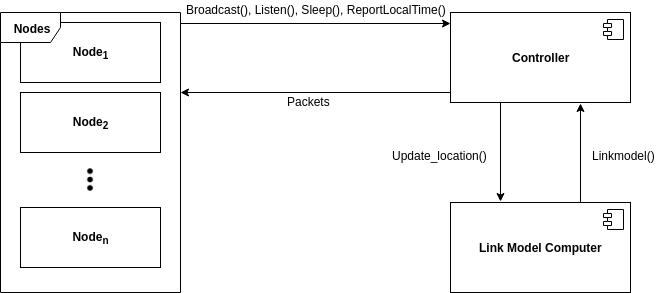
\includegraphics[width=0.8\textwidth]{figures/mpi_architecture.png}
    \caption{The architecture of the \acrlong{mpi}.}
    \label{figure:mpi_architecture}
\end{figure}

% Explain the scenario, why do we need this?

\section{Hardware Emulation}\label{sec:mpiprotocol}
In this section, we will introduce the hardware functions required to emulate the radio hardware on a wireless sensor node. The three essential functions for hardware emulation is: broadcasting (\autoref{algo:hwfuncstransmit}), listening (\autoref{algo:hwfuncslisten}), and sleeping (\autoref{algo:hwfuncssleep}). Additionally, a function for reporting the current local time (\autoref{algo:hwfuncsupdatelocaltime}) to the controller is added. This function should be used whenever none of the above functions are applicable, and will allow the controller to continue processing requests from other nodes.

%as well as a sample protocol that we can implement, using these functions. 

%\autoref{sec:saloha} will present the Slotted ALOHA protocol, and \autoref{sec:hwfuncspseudo} will present the three functions, along with pseudocode descriptions of these.

%\subsection{Hardware Functions}\label{sec:hwfuncspseudo}


\begin{algorithm}[ht]
    \DontPrintSemicolon
    \SetAlgorithmName{Data Structure}{Data Structure}

    \textbf{Structure} Message \{ action, source, localtime, duration, data \}\;
    \;
    clock $\leftarrow$ \Now\;
    localtime $\leftarrow$ 0\;
    id $\leftarrow$ unique identifier\;
 
    \caption{The shared variables and structures used by the hardware functions.}
    \label{algo:protocolsharedstate}
\end{algorithm}

\todo[inline]{fix autoref for data structure}
\todo[inline]{fix ref for virtual time}

The shared state for the hardware functions consist of three variables (\autoref{algo:protocolsharedstate}): \texttt{clock}, \texttt{localtime}, and \texttt{id}. The \texttt{clock} variable is used to measure the real-time spent by the node, between calls to the hardware function. \texttt{localtime} is used to track the local time of the node, as well as to enable virtual time (introduced in \autoref{sec:virtualtime}). Finally the \texttt{id} variable is a unique identifier assigned to each particular node. A common element for all of the hardware functions is that we initially update the \texttt{localtime} variable with the elapsed time since the \texttt{clock} variable was reset last, before transmitting the current local time, as well as a duration, to the controller. The \texttt{clock} variable is reset at the end of all of the functions, after an acknowledgement has been received from the controller.\medbreak

\begin{algorithm}[ht]
    \DontPrintSemicolon
    \KwResult{The time it took to broadcast the packet}
    \SetKwFunction{FBroadcast}{Broadcast}
    \SetKwProg{Fn}{Function}{}{}
    
    \Fn{\FBroadcast{packet}}{
        localtime $\leftarrow$ (\Now $-$ clock) $+$ localtime\;
        duration $\leftarrow$ transmission\_time(|packet|)\;
        m $\leftarrow$ \{ transmit, id, localtime, duration, packet \}\;
        \Send m \KwTo controller\;
        localtime $\leftarrow$ \Await ack \From controller\;
        clock $\leftarrow$ \Now\;
        \KwRet duration\;
    }

    \caption{The Broadcast Function.}
    \label{algo:hwfuncstransmit}
\end{algorithm}

The \texttt{Broadcast} (\autoref{algo:hwfuncstransmit}) function takes any arbitrary data packet, sends this to the controller using the \gls{mpi}, and waits for an acknowledgement from the controller. The controller takes care of distributing the packet to neighbouring nodes, including computing the probability of the neighbouring node receiving the packet. The duration required for transmitting a packet is computed using the baudrate, as specified by the hardware parameters described in \autoref{sed:baudrate}. This is sent to the controller, along with the packet, and we wait for an acknowledgement from the controller, containing our new local time.\medbreak
\todo[inline]{fix ref for baudrate}

\begin{algorithm}[ht]
    \DontPrintSemicolon
    \KwResult{list of packets}
    \SetKwFunction{FListen}{Listen}
    \SetKwProg{Fn}{Function}{}{}
    
    \Fn{\FListen{duration}}{
        localtime $\leftarrow$ (\Now $-$ clock) $+$ localtime\;
        m $\leftarrow$ \{ listen, id, localtime, duration \}\;
        \Send m \KwTo controller\;

        packets $\leftarrow$ empty list\;
        c $\leftarrow$ \Await count \From controller\;
        \For{i $\leftarrow$ 0 \KwTo c}{
            p $\leftarrow$ \Await packet \From controller\;
            \Append p \KwTo packets\;
        }

        localtime $\leftarrow$ \Await ack \From controller\;
        clock $\leftarrow$ \Now\;
        \KwRet packets\;
    }
    
    \caption{The Listen Function.}
    \label{algo:hwfuncslisten}
\end{algorithm}

The \texttt{Listen} (\autoref{algo:hwfuncslisten}) function takes a duration, and sends this, along with the updated local time, to the controller. The controller will return any packets the listening node have received within the duration, as well as an acknowledgement containing the new local time of the node.\medbreak

\begin{algorithm}[ht]
    \DontPrintSemicolon
    \SetKwFunction{FSleep}{Sleep}
    \SetKwProg{Fn}{Function}{}{}
    
    \Fn{\FSleep{duration}}{
        localtime $\leftarrow$ (\Now $-$ clock) $+$ localtime\;
        m $\leftarrow$ \{ sleep, id, localtime, duration \}\;
        \Send m \KwTo controller\;
        localtime $\leftarrow$ \Await ack \From controller\;
        clock $\leftarrow$ \Now\;
    }
    
    \caption{The Sleep Function.}
    \label{algo:hwfuncssleep}
\end{algorithm}

The \texttt{Sleep} (\autoref{algo:hwfuncssleep}) function also takes an duration, and sends this, along with the updated local time to the controller. The controller will send an acknowledgement containing the new local time of the node.\medbreak

\begin{algorithm}[ht]
    \DontPrintSemicolon
    \SetKwFunction{FReportLocalTime}{ReportLocalTime}
    \SetKwProg{Fn}{Function}{}{}
    
    \Fn{\FReportLocalTime{}}{
        localtime $\leftarrow$ (\Now $-$ clock) $+$ localtime\;
        m $\leftarrow$ \{ report-localtime, id, localtime \}\;
        \Send m \KwTo controller\;
        clock $\leftarrow$ \Now\;
    }
    
    \caption{The ReportLocaltime Function.}
    \label{algo:hwfuncsupdatelocaltime}
\end{algorithm}

Finally, the \texttt{ReportLocalTime} (\autoref{algo:hwfuncsupdatelocaltime}) function is included in the case where none of the above hardware functions are applicable. The function will send a message to the controller with the updated local time, and reset the \texttt{clock} variable.
\section{Centralised Controller}\label{sec:mpicontroller}
To facilitate communication between nodes using the hardware interface, we introduce a centralised controller. The centralised controller works by gathering requests (broadcasting, listening, or sleeping) from all nodes, and processing these.\medbreak

The controller works by continuously awaiting requests from any of the nodes in the network on \autoref{line:action-await}. A call of any of the hardware functions described in \autoref{sec:mpiprotocol} will result in a message arriving at the controller. Whenever a message has been received, the controller will update the local time of the sending node in the \texttt{nodes} variable on \autoref{line:action-updatelocaltime}. We keep track of the currently known local times for all nodes in order to know when we are ready to process listen requests. \smallbreak

If the request is a transmit request (\autoref{line:action-transmit}), we add the request to the \texttt{transmissions} list, to be processed later, and we send an acknowledgement packet to the transmitting node, containing the new local time for that node. Should the request be a listen request (\autoref{line:action-listen}), we instead add the request to the \texttt{listens} list. We do not acknowledgement the listen request at this state. Finally, is the request a sleep request (\autoref{line:action-sleep}), we immediately send an acknowledgement to the node, containing the updated local time. Note that any call to the \texttt{ReportLocalTime} function is handled at \autoref{line:action-updatelocaltime}, as this function does not require any acknowledgement.\smallbreak

After processing the message, we compute the minimum local time of all the nodes stored in the \texttt{nodes} variable on \autoref{line:mintime}. The \texttt{mintime} is used to check whether we are ready to process any of the listen requests stored in the \texttt{listens} variable. We iterate through these on \autoref{line:iterlistens} and check if the end of the listen interval is greater than the minimum local time computed earlier. If this is the case, or if the listen request has already been processed, we continue iterating through the list. Otherwise, we begin iterating each transmission request stored in the \texttt{transmissions} list on \autoref{line:itertransmissions}, and if the transmission interval is within the current listen interval (\autoref{line:iswithin}), we check if the packet should be received by the listening node by calling the \texttt{ShouldReceive} function, and if yes, we add the packet to the list of packets to be sent to the listening node. We send the packets to the listening node on \autoref{line:sendpackets}, followed by an acknowledgement containing the updated local time of the node.\medbreak

\todo[inline]{add pseudocode for the ShouldReceive function}
\begin{algorithm}[H]
    \DontPrintSemicolon
    \SetKwFunction{FController}{Controller}
    \SetKwProg{Fn}{procedure}{}{}
    
    \textbf{Structure} Message \{ action, source, localtime, duration, data \}\;
    \textbf{Structure} Transmission \{ source, start, end, data \}\;
    \textbf{Structure} Listen \{ source, start, end, processed \}\;
    \textbf{Structure} Node \{ localtime \}\; % location
    \;
    
    \Fn{\FController{}}{   
        transmissions $\leftarrow$ empty Transmission list\;
        listens $\leftarrow$ empty Listen list\;
        nodes $\leftarrow$ map containing all nodes with id as key\;
        \;
        \Repeat{\textit{protocol terminates}}{
            m $\leftarrow$ \Await Message \From any node\; \label{line:action-await}
            nodes(m.source).localtime $\leftarrow$ m.localtime + m.duration\; \label{line:action-updatelocaltime}

            \If{m.action = transmit}{ \label{line:action-transmit}
                t $\leftarrow$ \{ m.source, m.localtime, m.localtime $+$ m.duration, m.data \}\;
                \Append t \KwTo transmissions\;
                \Send nodes(m.source).localtime \KwTo node.id \tcp{ack}
            }
            \ElseIf{m.action = listen}{ \label{line:action-listen}
                l $\leftarrow$ \{ m.source, m.localtime, m.localtime $+$ m.duration, false \}\;
                \Append l \KwTo listens\;
            }
            \ElseIf{m.action = sleep}{ \label{line:action-sleep}
                \Send nodes(m.source).localtime \KwTo node.id \tcp{ack}
            }

            mintime $\leftarrow \min_{\forall \text{n} \in \text{nodes}}$(n.localtime)\; \label{line:mintime}

            \ForEach{l $\in$ listens}{ \label{line:iterlistens}
                \If{l.end $>$ mintime \Or l.processed}{
                    \Continue
                }

                packets $\leftarrow$ empty Packet list\;

                \ForEach{t $\in$ transmissions}{ \label{line:itertransmissions}
                    \If{t.id $=$ l.id}{
                        \Continue
                    }

                    \If{t.start $\geq$ l.start \And t.end $\leq$ l.end}{ \label{line:iswithin}
                        \If{ShouldReceive(t.id, l.id, transmissions)}{ \label{line:shouldreceive}
                            \Append t.data \To packets\;
                        }
                    }
                }

                \Send $|$packets$|$ \To l.id\; \label{line:sendcount}                   
                
                \ForEach{p $\in$ packets}{ \label{line:sendpackets}
                    \Send p \To l.id\;
                }

                \Send nodes(l.id).localtime \KwTo l.id \tcp{ack}
                l.processed $\leftarrow$ true\;
            }


        }
    }
    \caption{The Controller procedure.}
    \label{algo:mpicontroller}
\end{algorithm}

















%The centralised controller consist of two concurrent procedures. The \texttt{MessageHandler} procedure (\autoref{algo:mpimessagehandler}), and the \texttt{Controller} procedure (\autoref{algo:mpicontrollerpart}). A shared state is used to manage the data between the two procedures (\autoref{algo:mpisharedstate}). \medbreak
%\todo[inline]{fix autoref for data structure}

%In essence, the centralised controller works by gathering all requests from all nodes in the \texttt{MessageHandler} procedure for a given time slot, and by processing, and responding to the requests in the \texttt{Controller} procedure.

% \begin{algorithm}[ht]
%     \DontPrintSemicolon
%     \SetAlgorithmName{Data Structure}{Data Structure}
    
%     \textbf{Structure} Message \{ action, source, localtime, duration, data \}\;
%     \textbf{Structure} Transmission \{ source, start, end, data \}\;
%     \textbf{Structure} Listen \{ source, start, end, processed \}\;
%     \textbf{Structure} Node \{ localtime \}\; % location
%     \;
    
%     queue $\leftarrow$ empty Message queue\;
%     transmissions $\leftarrow$ empty Transmission list\;
%     listens $\leftarrow$ empty Listen list\;

%     nodes $\leftarrow$ map containing all nodes with id as key\;
%     %transmissions $\leftarrow$ empty map\;
 
%     \caption{The shared state variables and structures used by the controller.}
%     \label{algo:mpisharedstate}
% \end{algorithm}

%The shared state consists of two structures, \texttt{Message} and \texttt{Node}, used to store messages and nodes respectively, as well as three global variables: \texttt{nodes}, \texttt{transmissions}, and \texttt{currenttime}. \smallbreak

%\texttt{nodes} is a map of key-value pairs, containing every node in the network, with the unique identifier of the node as the key, and a \texttt{Node} structure as the value. \smallbreak

%\texttt{transmissions} is another map of key-value pairs, where the key is the unique identifier of a transmitting node, and the value is the data packet sent from the node. \smallbreak

%\texttt{currenttime} is an integer used to keep track of the already processed time slots, whenever a time slot has been processed, this is incremented.

%\begin{algorithm}[ht]
%    \DontPrintSemicolon
%    \SetKwFunction{FMessageHandler}{MessageHandler}
%    \SetKwProg{Fn}{procedure}{}{}
%    
%    \Fn{\FMessageHandler{}}{
%        \Repeat{\textit{protocol terminates}}{
%            m $\leftarrow$ \Await Message \From any node\;
%        
%            \If{m.action = transmit}{
%                nodes(m.source).time $\leftarrow$ nodes(m.source).time + 1\;
%                nodes(m.source).state $\leftarrow$ transmitting\;
%                transmissions(m.source) $\leftarrow$ m.data\;
%            }
%            \ElseIf{m.action = listen}{
%                nodes(m.source).time $\leftarrow$ nodes(m.source).time + m.time\;
%                nodes(m.source).state $\leftarrow$ listening\;
%            }
%            \ElseIf{m.action = sleep}{
%                nodes(m.source).time $\leftarrow$ nodes(m.source).time + m.time\;
%                nodes(m.source).state $\leftarrow$ sleeping\;
%            }
            %\ElseIf{m.action = location}{
            %    nodes(m.source).location $\leftarrow$ m.data as location\;
            %}
%        }
%    }
%    \caption{The MessageHandler procedure.}
%    \label{algo:mpimessagehandler}
%\end{algorithm}



%The task of the \texttt{MessageHandler} procedure is to continuously gather requests from all of the nodes in the network, and change the state and local time of the node in the \texttt{nodes} map, as well as storing the data packet for any transmitting node in the \texttt{packets} map. \medbreak

%Whenever requests have been gathered from all nodes for a time slot, we are able to process the time slot. This is the task of the \texttt{Controller} procedure. On \autoref{line:awaitprocess} in \autoref{algo:mpicontrollerpart}, we wait until every node in the \texttt{nodes} map has a $\texttt{time} > \texttt{currenttime}$, which means that every node has sent a request for the \texttt{currenttime}'th time slot. If this is the case, we are able to process the time slot. A time slot is processed by first iterating through all nodes that are either in the \texttt{transmitting} or \texttt{sleeping} state. If the node is transmitting, we need to distribute the packet to all neighbours of the node that are able to receive the packet, by adding the packet to the \texttt{packets} list in the \texttt{Node} structure. This is decided by the link model (TODO), where we compute the probability of the neighbour receiving the packet, as described in \autoref{sec:linkmodel}. Is the node currently sleeping, we send a wakeup message to the node, if the local time of the node is equal to our \texttt{currenttime} variable. \smallbreak

%\todo[inline]{Incorporate link model}

%After processing any transmitting or sleeping nodes, we iterate through the map of nodes once again, but this time we process any nodes currently listening for packets. If the local time of the node listening for packets is equal to our \texttt{currenttime} variable, we send any packets stored in the \texttt{packets} list of the node, and clear the contents of the list afterwards.

% \begin{algorithm}[ht]
%     \DontPrintSemicolon
%     \SetKwFunction{FProcessor}{Controller}
%     \SetKwProg{Fn}{procedure}{}{}
    
%     \Fn{\FProcessor{}}{
%         \Repeat{\textit{protocol terminates}}{
%             \Await every node $\in$ nodes, where node.time $>$ currenttime\;\label{line:awaitprocess}
            
%             currenttime $\leftarrow$ currenttime + 1\;
        
%             \ForEach{node $\in$ nodes}{
%                 \If{node.state = transmitting}{
%                     %m $\leftarrow$ Message\;
%                     %m.action $\leftarrow$ transmit\;
%                     data $\leftarrow$ transmissions(node.id)\;
                    
%                     \ForEach{neighbour $\in$ neighbours(node)}{
%                         \If{neighbour.state = listening \And shouldreceive(neighbour)}{
%                             \Append data \KwTo neighbour.packets\;
%                         }
%                     }
                    
%                     \Remove transmissions(node.id)\;
%                     \Send ack \KwTo node.id\;
%                 }
%                 \ElseIf{node.state = sleeping \And node.time = currenttime}{
%                     \Send wakeup \KwTo node.id\;
%                 }
%             }
            
%             \ForEach{node $\in$ nodes}{
%                 \If{node.state = listening \And node.time = currenttime}{
%                     \Send $|$node.packets$|$ \KwTo node.id\;                
%                     \ForEach{packet $\in$ node.packets}{
%                         \Send packet \KwTo node.id\;
%                     }
                    
%                     \Clear node.packets\;
%                 }
%             }
        
%         }
%     }
    
%     \caption{The Controller procedure.}
%     \label{algo:mpicontrollerpart}
% \end{algorithm}


\section{Link Model Computer}\label{sec:mpi:lmc}
% intro




%In \autoref{sec:mpinodelocation} we mentioned that the location of all nodes should be known by the controller, 

%The reason for introducing a separate compute node, dedicated to the link model, is to offload the controller. Both handling packets transmission, synchronising time and computing the link model is too much responsibility for a single node. Offloading also allows for simplifying the logic in the controller.

%When the network is initialized, the controller will transmit the current image of the network to the \gls{lmc}. The \gls{lmc} will then compute the link model based on the received information. During the simulation, the controller can update the stored network image. This allows for removing and adding nodes to the network, while also allowing the controller to update a nodes location data, thereby keeping an updated image of the network. The \gls{lmc} will first re-compute the link model, when an update has happened. When the simulation is to be stopped, the controller will notify the \gls{lmc}, and the compute node will terminate.
\section{Hardware Interface (hardware.h)}\label{sec:hardwareinterface}
In this section we will describe the design of the hardware (\gls{lowerlayer}) interface, used by an \gls{upperlayer} protocol to simulate radio communication between nodes in a \gls{manet}. The section will serve as the documentation, as well as a programmers guide, for the \mintinline{cpp}{hardware.h} interface.\medbreak

The hardware interface is implemented in modern C++, using templates, which will allow a protocol implementation to transmit instances of arbitrary structures or classes between nodes, provided that the structure or class is a trivially copyable type~\cite{website:cpptriviallycopyable}.

\begin{description}[style=nextline,leftmargin=0cm]
    \item[\mintinline{cpp}{void hardware::init(const Location &loc)}]
        Initialises the hardware functionality by initialising the \gls{mpi} functionality, as well as registering the node with the \gls{mpi} controller. The location is stored on the controller, and can later be update by using the \mintinline{cpp}{set_location()} function. The location of a node is used to compute neighbourhood information, as well as the \gls{pathloss} experienced when transmitting data between nodes. This function has to be called exactly once, before calling any other hardware functions.
    
    \item[\mintinline{cpp}{void hardware::deinit()}]
        De-initialises the hardware functionality by un-registering the node from the \gls{mpi} controller, as well as de-initialising the \gls{mpi} functionality. This function has to be called exactly once, before terminating the protocol.
        
    \item[\mintinline{cpp}{template <typename T>}\\\mintinline{cpp}{std::chrono::microseconds hardware::broadcast(T &packet)}]
        Transmit a data packet of type \mintinline{cpp}{T}. \autoref{algo:hwfuncstransmit} contains a pseudo code description of this function. Returns the duration the transmission took, in microseconds.

    \item[\mintinline{cpp}{template <typename T>}\\\mintinline{cpp}{std::vector<T> hardware::listen(std::chrono::microseconds duration)}]
        Listen for data packets of type \mintinline{cpp}{T} for a given duration of microseconds. \autoref{algo:hwfuncslisten} contains a pseudo code description of this function.
    
    \item[\mintinline{cpp}{void hardware::sleep(std::chrono::microseconds duration)}]
        Sleep for a given duration of microseconds. \autoref{algo:hwfuncssleep} contains a pseudo code description of this function.

    \item[\mintinline{cpp}{void report_localtime()}]
        Report the current local time to the controller.    
    
    \item[\mintinline{cpp}{unsigned long hardware::get_id()}]
        Gets the unique identifier of the node, assigned by the \gls{mpi} library. This function will return 0, if the \mintinline{cpp}{init_hardware()} function has not yet been called.
    
    \item[\mintinline{cpp}{unsigned long hardware::get_world_size()}]
        Gets the total amount of nodes registered to the \gls{mpi} controller. This function will return 0, if the \mintinline{cpp}{init_hardware()} function has not yet been called.
    
    \item[\mintinline{cpp}{bool hardware::set_location(const Location &loc)}]
        Updates the location registered on the \gls{mpi} controller. Returns \mintinline{cpp}{true} if the location was successfully updated, and \mintinline{cpp}{false} if the location update failed on the controller, or if the \mintinline{cpp}{init_hardware()} function has not yet been called.

\end{description}

A sample implementation of the Slotted ALOHA protocol using the hardware interface described above, can be found at \autoref{minted:cpp:slottedaloha} in \autoref{app:slottedaloha}.
